\documentclass{article}
\usepackage{geometry}
\usepackage[table]{xcolor}% http://ctan.org/pkg/xcolor
\usepackage{fancyhdr}
\usepackage{amsmath, amssymb}
\usepackage{graphicx}
\usepackage{color}
\usepackage{longtable}
\definecolor{bg}{rgb}{0.89, 0.95, 0.71} % background e3f3b4
\definecolor{ac}{rgb}{0.50, 0.18, 0.41} % accent c491b6
\definecolor{rc}{rgb}{0.77, 0.57, 0.71} % rule 7f2f69
\usepackage{listings}
%catalan packages
\usepackage[catalan]{babel}
\usepackage[T1]{fontenc}
\usepackage[utf8]{inputenc}
%
\lstset{
       basicstyle=\small\ttfamily,
       xleftmargin=1em,
       }
\lstdefinestyle{latex}{language=TeX,
                       backgroundcolor=\color{bg},
                       basicstyle=\small\ttfamily,
                       frame=leftline,
                       xleftmargin=1.4em,
                       framexleftmargin=.8em}
\lstdefinestyle{cmdline}{
                         }
\usepackage{url}
\usepackage[pdftex,
            bookmarks,
            colorlinks=true,
            linkcolor=black,
            plainpages = false,
            pdfpagemode = UseNone,
            pdfstartview = FitH,
            citecolor = ac, urlcolor = ac, filecolor = ac]{hyperref}

\usepackage[para]{footmisc}
% Change horiz room between fn mark and fn hskip from .5em
% Suggested to RF making this settable
\makeatletter
\long\def\@makefntext#1{\leavevmode
\@makefnmark\nobreak
\hskip.05em\relax#1%
}
\makeatother
%\newcommand{\texdoc}[1]{\/\footnote{\protect\texttt{#1}}}
\newcommand{\citelink}[3]{\href{#1}{#2}~\cite{#3}}
\newcommand{\bibliolink}[2]{\href{#1}{\nolinkurl{#1}}, \href{#1}{#2}}

\setlength{\parskip}{0.75ex}
\makeatletter 
\makeatother
\setcounter{secnumdepth}{0}

\newlength{\rulelength}
\setlength{\rulelength}{\linewidth}
\addtolength{\rulelength}{9.5em}
\addtolength{\oddsidemargin}{-1in}
\addtolength{\evensidemargin}{-1in}
\title{Must Know}
\author{INS Vilafant 18/19}
\date{\today}

\pagestyle{plain}
\begin{document}
\thispagestyle{empty}
%\maketitle
\setlength{\unitlength}{1in}

\makeatletter
%\vspace*{3ex}
\par\noindent{\LARGE\bf \@title}
\vspace*{-1.2ex}
\par\noindent{{\rule{\textwidth}{1.05pt}}}
%\vspace*{-.5ex}
\par\noindent{\large \@author}
%\vspace*{5ex}
%\makeatother
\section{Successions}
\begin{itemize}
	\item Aritmètica: $a_n=a_1 + (n-1)\cdot d$
	\item Geomètrica: $a_n=a_1 \cdot r^{n-1}$ 
\end{itemize}

\section{Àrea de figures planes}

\begin{tabular}{|l|l|}
\hline
Quadrat	& $A_{Q}=c^2$  \\
\hline
Rectange	& $A_{R}=b\cdot h$ \\
\hline
Triangle	& $A_{T}=\frac{b\cdot h}{2}$\\
\hline
Polígon regular	& $A_{PR}=\frac{perim\cdot apotema}{2}$\\
\hline
Rombe	& $A_{RB}=\frac{D\cdot d}{2}$\\
\hline
Trapezi	& $A_{TP}=\frac{(B+b)\cdot h}{2}$\\
\hline
Cercle	& $A_{C}=\pi \cdot r^2$\\
\hline
\end{tabular} 

\section{Àrees i volums de cossos geomètrics}

\begin{tabular}{|l|l|}
 \hline
Cub& $A_{cub}=6\cdot c^2 \qquad V_{cub}=c^3$ \\
\hline
Prisma& $A_{prisma}=2\cdot A_{base}+n\cdot A_{rec. lat.} \qquad V_{prisma}=a\cdot b \cdot c$ \\
\hline
Piràmide& $A_{piramide}=A_{base}+n\cdot A_{triang. lat.} \qquad V_{piramide}=\frac{1}{3} A_{base} \cdot h$\\
\hline
Cilindre& $A_{cilindre}=2 \cdot \pi r^2+2\cdot \pi \cdot r \cdot h \qquad V_{cilindre}=\pi \cdot r^2 \cdot h$\\
\hline
Con& $A_{con}=\cdot \pi r^2+ \pi \cdot r \cdot g \qquad V_{con}=\frac{1}{3}\pi \cdot r^2 \cdot h$\\
\hline
Esfera& $A_{esfera}=4 \cdot \pi r^2 \qquad V_{esfera}=\frac{4}{3}\pi \cdot r^3$\\
\hline  
\end{tabular}

\section{Identitats notables}
\begin{itemize}
	\item Quadrat d'una suma: $(a+b)^2=a^2+b^2+2ab$
	\item Quadrat d'una diferència: $(a-b)^2=a^2+b^2-2ab$
	\item Suma per diferència: $(a+b)\cdot(a-b)=a^2-b^2$
\end{itemize}
\newpage
\section{Descomposició factorial de polinomis}

\begin{enumerate}
	\item Treure factor comú
	\item Identificar identitats notables
	\item Descomposició per Ruffini $(x-a)$
\end{enumerate}

\section{Representació gràfica de funcions}

\begin{tabular}{|l|l|}
	\hline 
	Domini& $\begin{cases} \frac{f(x)}{g(x)}\rightarrow D=\mathbb{R}-zeros\qquad g(x)\\ \sqrt{f(x)}\rightarrow D=x | f(x) \ge 0\\ log(f(x)) \rightarrow D=x | f(x) > 0 \end{cases}$\\
	\hline
	Punts de tall amb els eixos& eix $x\rightarrow f(x)=0$, eix $y\rightarrow f(0)$\\
	\hline
	Simetries&Parell: $f(x)=f(-x)$,  Senar $f(x)=-f(-x)$\\
	\hline
	Ass. verticals& $\rightarrow \lim_{x\to a }f(x)=\pm \infty$\\
	\hline
	Ass. horitzontals& $\rightarrow \lim_{x\to \pm \infty }f(x)=a$\\
	\hline
	Creixement i decreixement& $\rightarrow$ signe $f^{\prime}(x)$\\
	\hline
	Màxims i mínims& $\rightarrow$ $f^{,}(x)=0$ i $f^{,,}(x)<0$ o $f^{,,}(x)>0$\\
	\hline
	Punts d'inflexió& $\rightarrow$ $f^{,,}(x)=0$ i $f^{,,,}(x)\neq 0$\\
	\hline
	Concavitat i convexitat& $\rightarrow$ signe $f^{,,}(x)$\\
	\hline
	\multicolumn{2}{|c|}{\textbf{Translacions en els eixos}}\\
	\hline
	Eix x& $f(x+a), a>0\rightarrow$ Trasllada $f(x)$ $a$ unitats cap a l'esquerra \\
	\hline
	Eix y& $f(x)+a, a>0\rightarrow$ Trasllada $f(x)$ $a$ unitats cap a dalt\\
	\hline
\end{tabular}

\section{Rectes}


$y=mx+n$


$Ax+By-C=0\rightarrow \overrightarrow{v}=(-B,A)\qquad m=-\frac{A}{B}$

\section{Funció quadràtica}

\begin{minipage}{0.5\textwidth}
	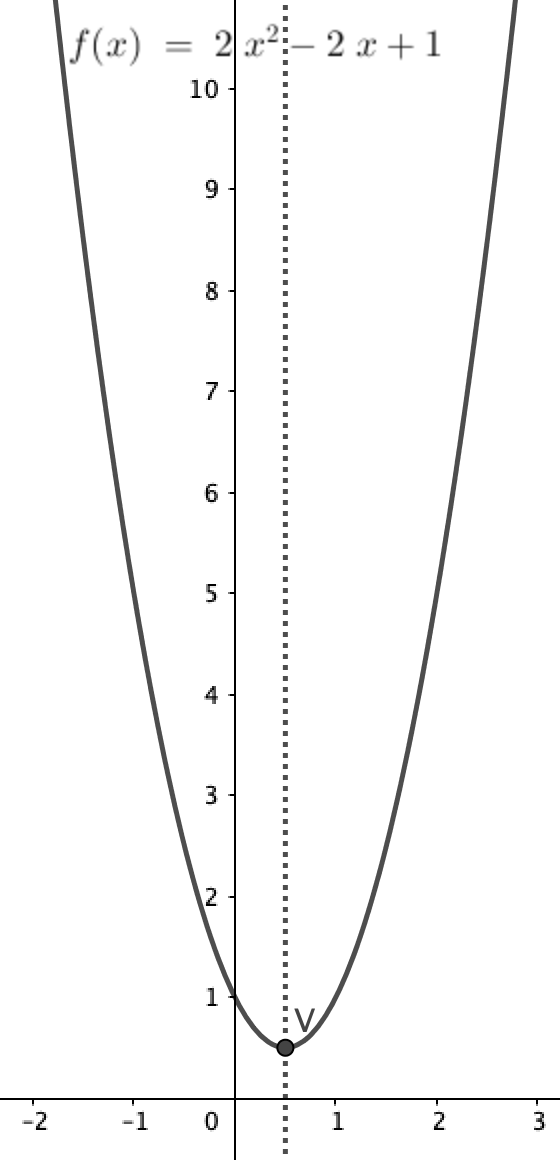
\includegraphics[width=0.4\textwidth]{eq_2n_grau.png}
\end{minipage}
\begin{minipage}{0.5\textwidth}
	 \vspace{0.5cm}
	$y=ax^2+bx+c$\\
	Vèrtex$\rightarrow x=-\frac{b}{2a}$\\
	Tall eix x: $ax^2+bx+c=0\rightarrow x=\frac{-b \pm \sqrt{b^2-4ac}}{2a}$\\
	Tall eix y: $(0,c)$\\
	$a>0\rightarrow \cup \qquad a<0\rightarrow \cap$\\
	
\end{minipage}

\section{Funció de proporcionalitat inversa}
\begin{minipage}{0.5\textwidth}
	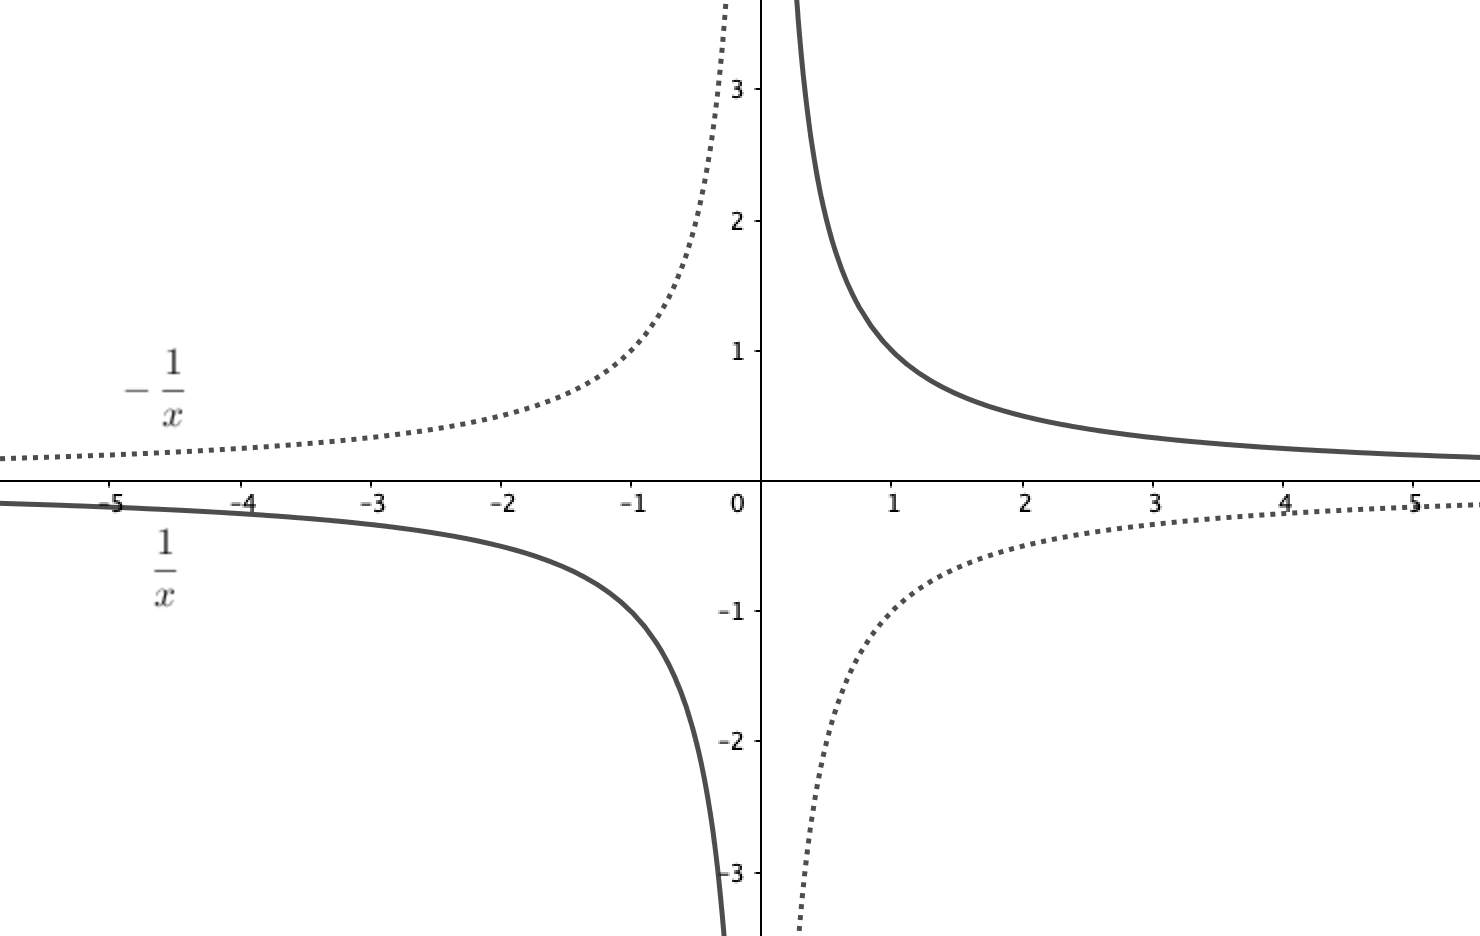
\includegraphics[width=0.6\textwidth]{funcio_prop_inversa.png}
\end{minipage}
\begin{minipage}{0.5\textwidth}
	\vspace{0.5 cm}
	$f(x)=\pm \frac{1}{x}$\\
\end{minipage}

\section{Funció exponencial}
\begin{minipage}{0.5\textwidth}
	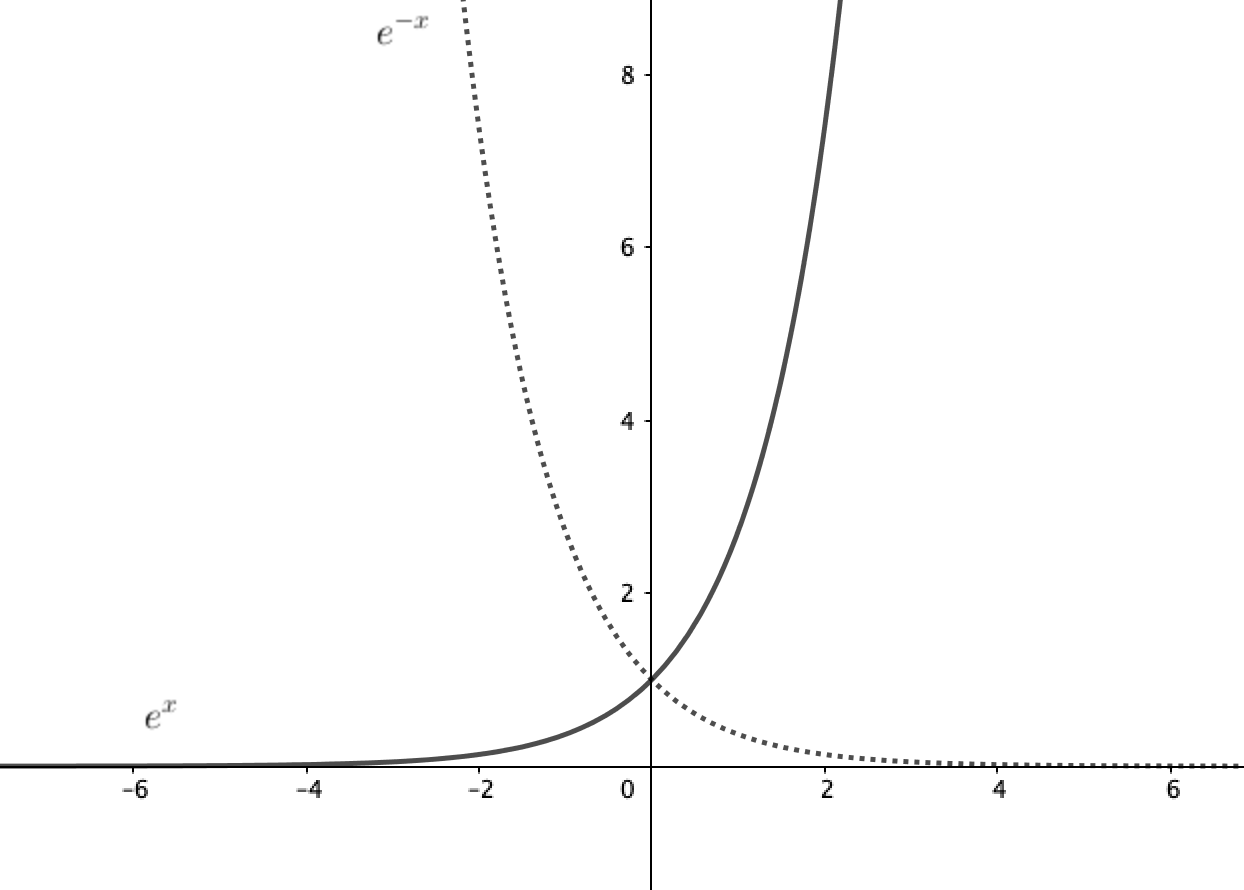
\includegraphics[width=0.6\textwidth]{funcio_exp.png}
\end{minipage}
\begin{minipage}{0.5\textwidth}
	\vspace{0.5 cm}
	$f(x)=e^{\pm x}$\\
\end{minipage}

\section{Funció logarítmica}
\begin{minipage}{0.5\textwidth}
	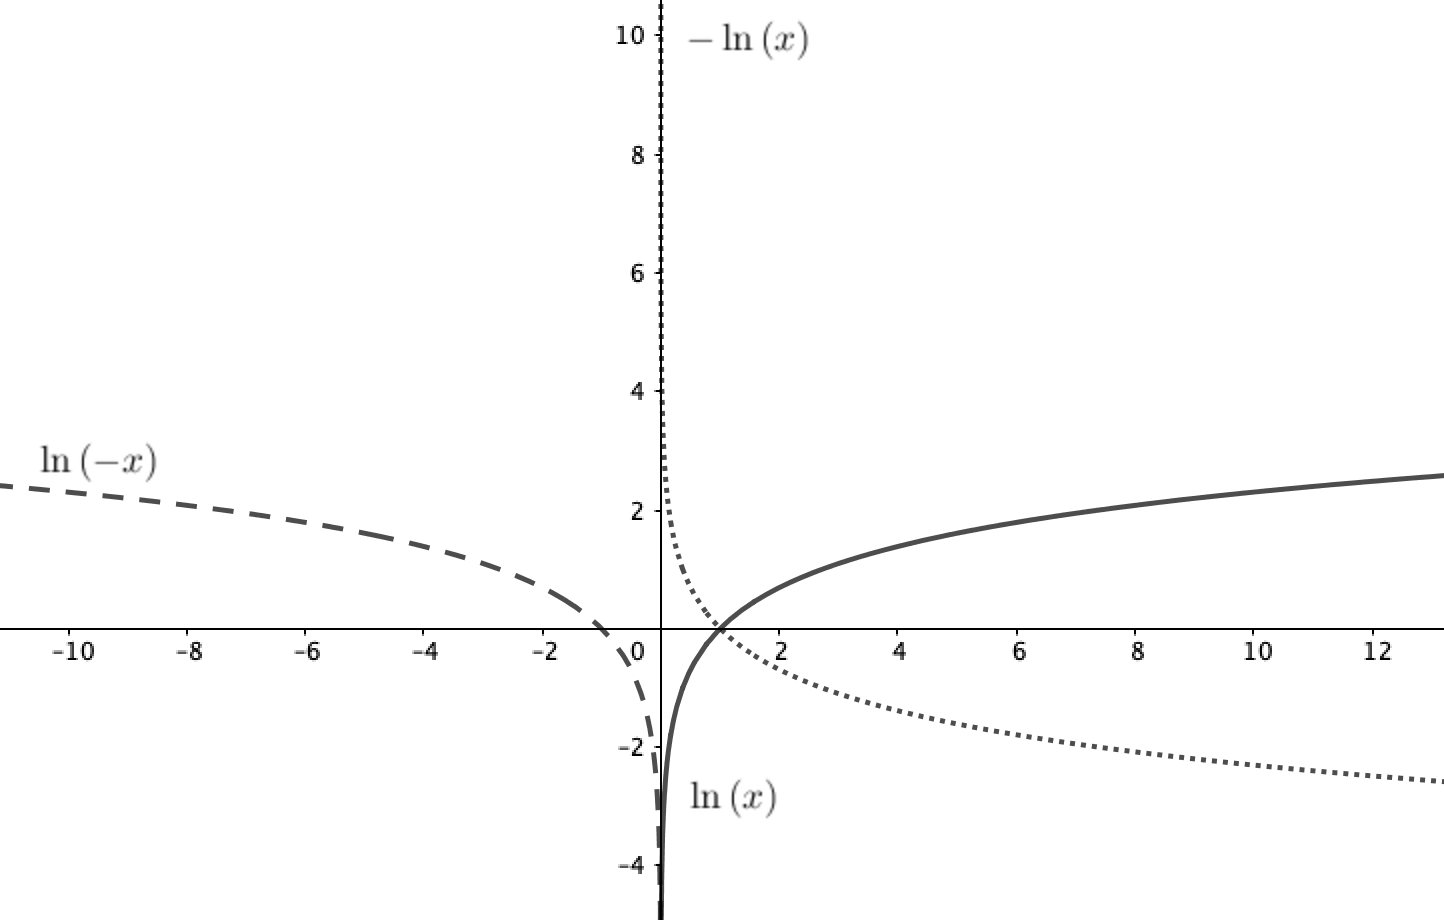
\includegraphics[width=0.6\textwidth]{funcio_ln.png}
\end{minipage}
\begin{minipage}{0.5\textwidth}
	\vspace{0.5 cm}
	$f(x)=\ln (\pm x)$\\
	$f(x)=-\ln (x)$\\
\end{minipage}

\section{Recta tangent a la gràfica d'una funció en un punt}
\begin{minipage}{0.5\textwidth}
	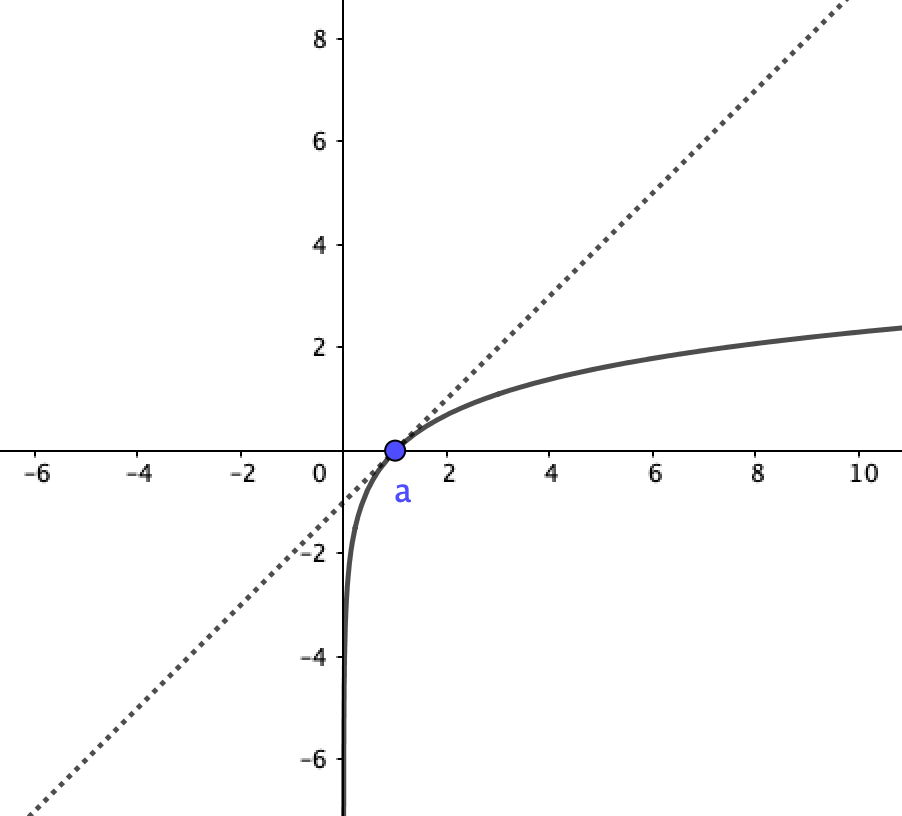
\includegraphics[width=0.6\textwidth]{recta_tangent.png}
\end{minipage}
\begin{minipage}{0.5\textwidth}
	\vspace{0.5 cm}
	$y-f(a)=f^{\prime}(a)(x-a)$\\
	
\end{minipage}

\section{Trigonometria}
\begin{minipage}{0.5\textwidth}
	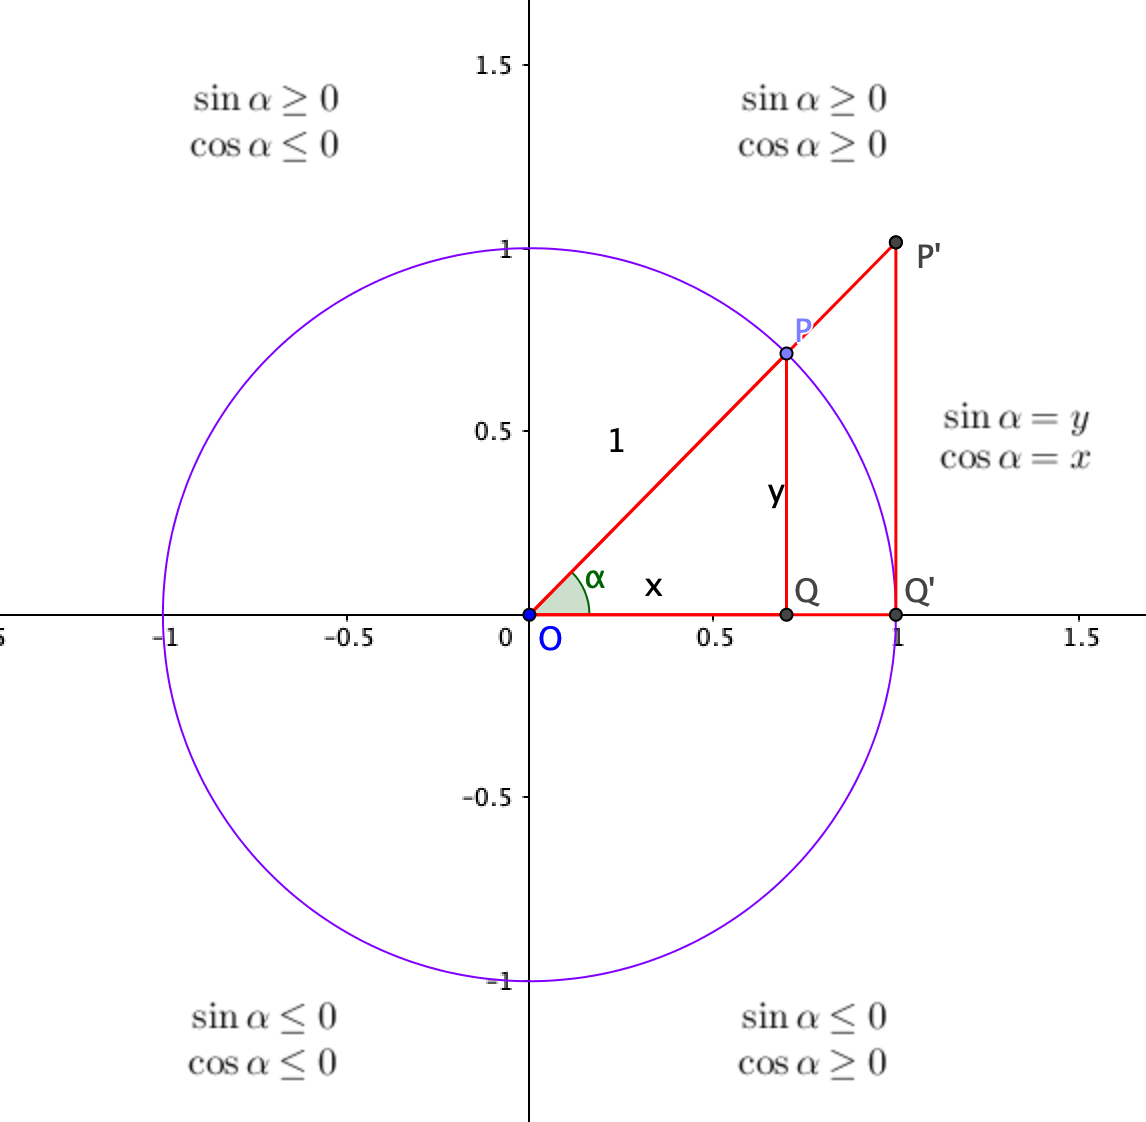
\includegraphics[width=0.6\textwidth]{circumf_unitat.png}
\end{minipage}
\begin{minipage}{0.5\textwidth}
	\vspace{0.5 cm}
	$\sin^2 x + \cos^2 x=1  $\\ 
	$\cos(2x) =\cos^2 x-\sin^2 x$\\
	$\sin(2x)=2\cos x \sin x$\\
	\end{minipage}
\end{document}
